%!TEX root = ../thesis.tex
%*******************************************************************************
%****************************** Third Chapter **********************************
%*******************************************************************************

\chapter{Feynman-Kac: connecting Quantum Mechanics and Stochastic Processes}
\label{chapter3}

% **************************** Define Graphics Path **************************
\ifpdf
    \graphicspath{{Chapter3/Figs/Raster/}{Chapter3/Figs/PDF/}{Chapter3/Figs/}}
\else
    \graphicspath{{Chapter3/Figs/Vector/}{Chapter3/Figs/}}
\fi

\section{Stochastic processes}
\label{subsec:fk-stoch}

\subsection{The Weiner process}
\begin{itemize}
	\item definition
	\item figure displaying it, alongside it figure of SDE for next section
\end{itemize}

\subsection{Stochastic Differential Equations and Ito Calculus}
\begin{itemize}
	\item Basic SDE
	\item Examples of famous cases (Ornstein-Uhlenbeck?)
	\item Ito calculus (the essentials)
	\item Fokker-Planck and the FP generator
\end{itemize}


\subsection{Discrete time Markov Chains}
More formally, the Markov process generator.

\subsection{Continuous time Markov Chains}
Rate matrix etc.

\subsection{Master equation}
Describes the time evolution of a system which can be described as a probabilistic combination of states and the transitions between these states is encapsulated with the \emph{transition rate matrix}.
\begin{equation}
	\partial_{t} \mathbf{P} = A \mathbf{P},
\end{equation}
where $A$ are the \emph{connections} and $\mathbf{P}$ are the probabilities.  

\section{The Feynman-Kac formula}
\label{subsec:fk-fk}
The Feynman path integral formulation~\eqref{eq:FPI} was extensively used by physicists for decades, even in the absence of a formal mathematical formulation which is hard to define because of the difficulties with defining an appropriate measure on the path space. Kac~\cite{kac1949distributions} provided a rigorous formulation of the \textit{real-valued} case of the Feynman path integral, and the resulting \emph{Feynman-Kac} formula provides a bridge between \emph{parabolic} partial differential equations and stochastic processes.

To illustrate the Feynman-Kac formula let us consider a single particle with Hamiltonian
\begin{equation}
	\hat{H} = -\frac{\mathrm{d}^2~~}{\mathrm{d}x^2} + V(x)
\end{equation}
and the Schr\" odinger equation in \textit{imaginary time}, which is of the elliptic type, 
\begin{equation}
	\label{eq:imag_sch}
	\partial_t | \psi_t \rangle = - \hat{H} | \psi_t \rangle.
\end{equation}
Its formal solution, the time propagation of an initial wave function $|\phi_0\rangle$ at $t=0$, is written as
\begin{equation}
	\left| \psi_{t} \right\rangle = e^{-\hat{H} t}\left|\psi_{0}\right\rangle. 
\end{equation}
From the spectral decomposition of the operator $e^{-\hat{H} t}$ in terms of eigenstates $|\phi_n\rangle$ and eigen-energies $E_n$ of the Hamiltonian $\hat{H}$
\begin{equation}
	e^{-\hat{H} t}=\sum_{n} e^{-E_{n} t}|\phi_n\rangle\langle\phi_n|, 
\end{equation}
it follows that the term corresponding to the ground state of the system $|\phi_0\rangle$ decays the slowest. Thus starting in some initial state and propagating for a long imaginary time $it$ leads into the ground state with the decay rate giving the ground state energy as
\begin{equation}
	\lim_{t \rightarrow \infty} | \psi_t \rangle \propto e^{-E_0 t} | \phi_0 \rangle,
\end{equation} 
where $E_0$ is the ground state energy and $|\phi_0\rangle$ is the corresponding state. Kac noticed that the kinetic term of the Lagrangian in~\eqref{eq:FPI} could be interpreted as a measure on Brownian walks, and a solution to the imaginary time Schr\" odinger equation can be written as
\begin{equation}
	\psi(x, t)=\underset{X \sim \text { Brownian with } X_{t}=x}{\mathbb{E}}
	\left[\exp \left(-\int_{0}^{t}  V\left(X_{\tau}, \tau \right) \mathrm{d}\tau \right) \psi\left(X_{0}, 0\right)\right],
\end{equation}
where only the \textbf{endpoint} at time $t$ of the Brownian process fixed, whereas the starting point at time $t=0$ is not, $\psi (x, 0)$ encodes the initial condition into this representation. When there is no external potential $V(x) = 0$, the Schr\" odinger equation in imaginary time is the diffusion equation and the Feynman-Kac solution is simply
\begin{equation}
	\begin{aligned} 
		\psi(x, t) &= \underset{X \sim \text { Brownian with } X_{t}=x}{\mathbb{E}}\left[\psi\left(X_{0}, 0\right)\right] \\
		&=  
		\frac{1}{\sqrt{2 \pi t}} \int  e^{-\left(x-x^{\prime}\right)^{2} / 2 t} \psi_{0}\left(x^{\prime}\right) \mathrm{d} x^{\prime}
	\end{aligned}
\end{equation}
An illustration of the Feynman-Kac approach to the problem with no external potential $V(x)$ in 1D is depicted in Fig.~\ref{fig:fk_1d_example}.
\begin{figure}[H]
	\centering
	\subfloat
	{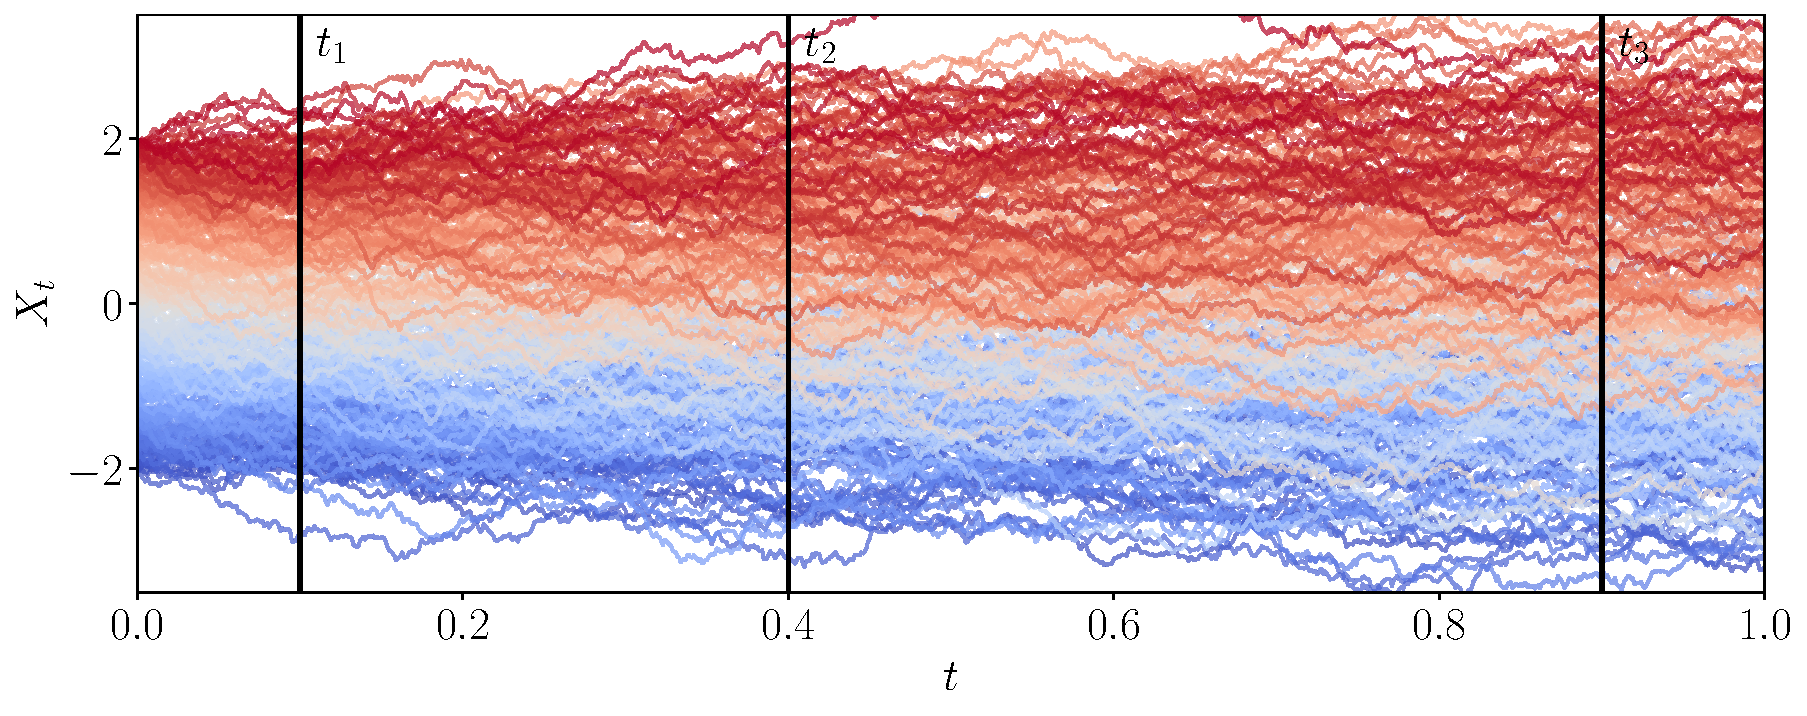
\includegraphics[width = \linewidth]{Chapter2/Figs/Raster/fkac_vs_fplanck_top.pdf}} \\
	\subfloat
	{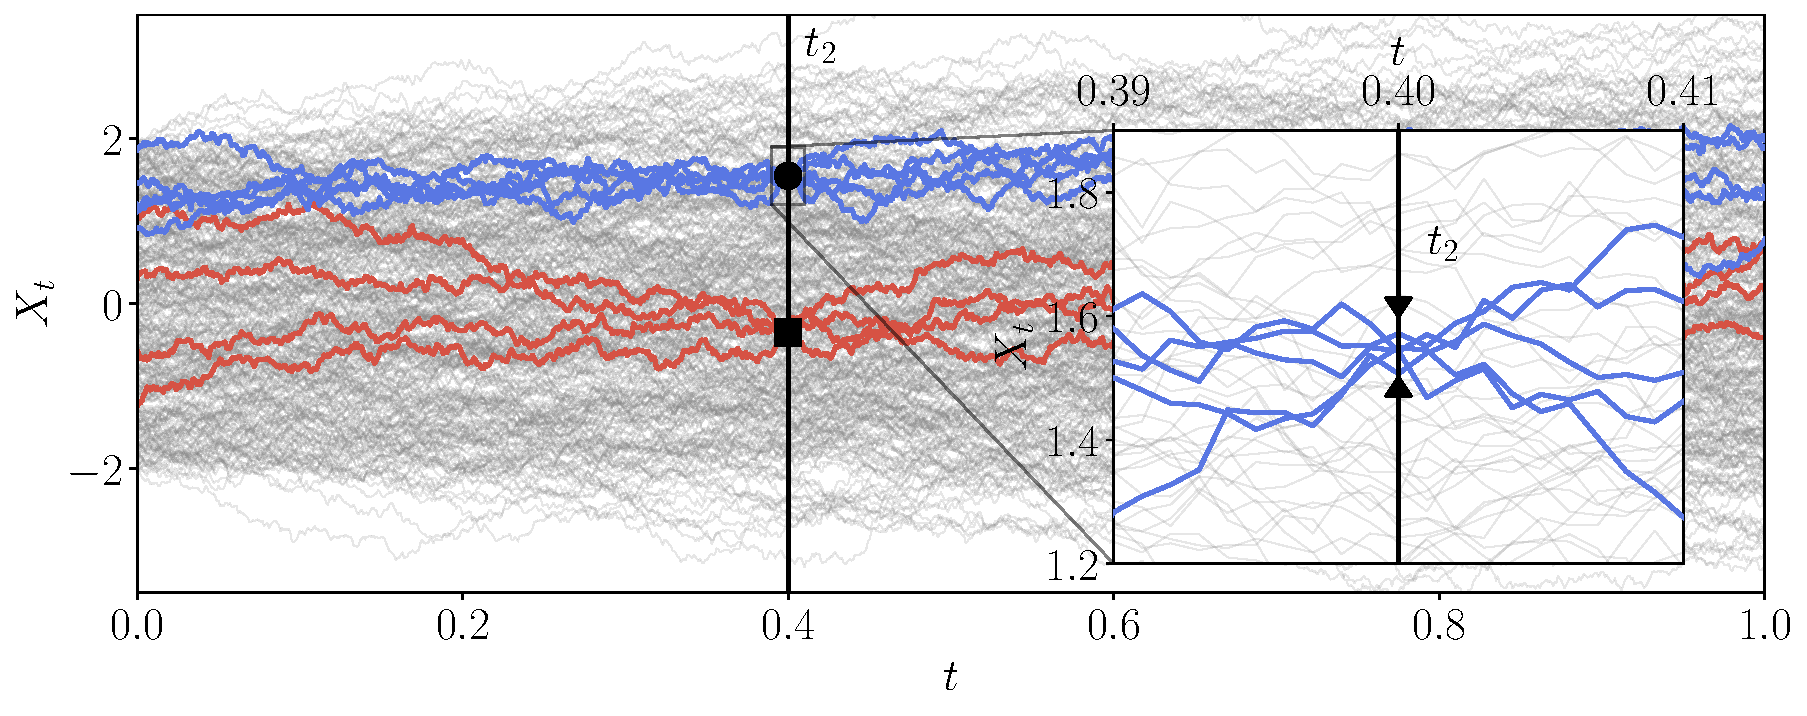
\includegraphics[width = \linewidth]{Chapter2/Figs/Raster/fkac_vs_fplanck_mid1.pdf}} \\
	\subfloat
	{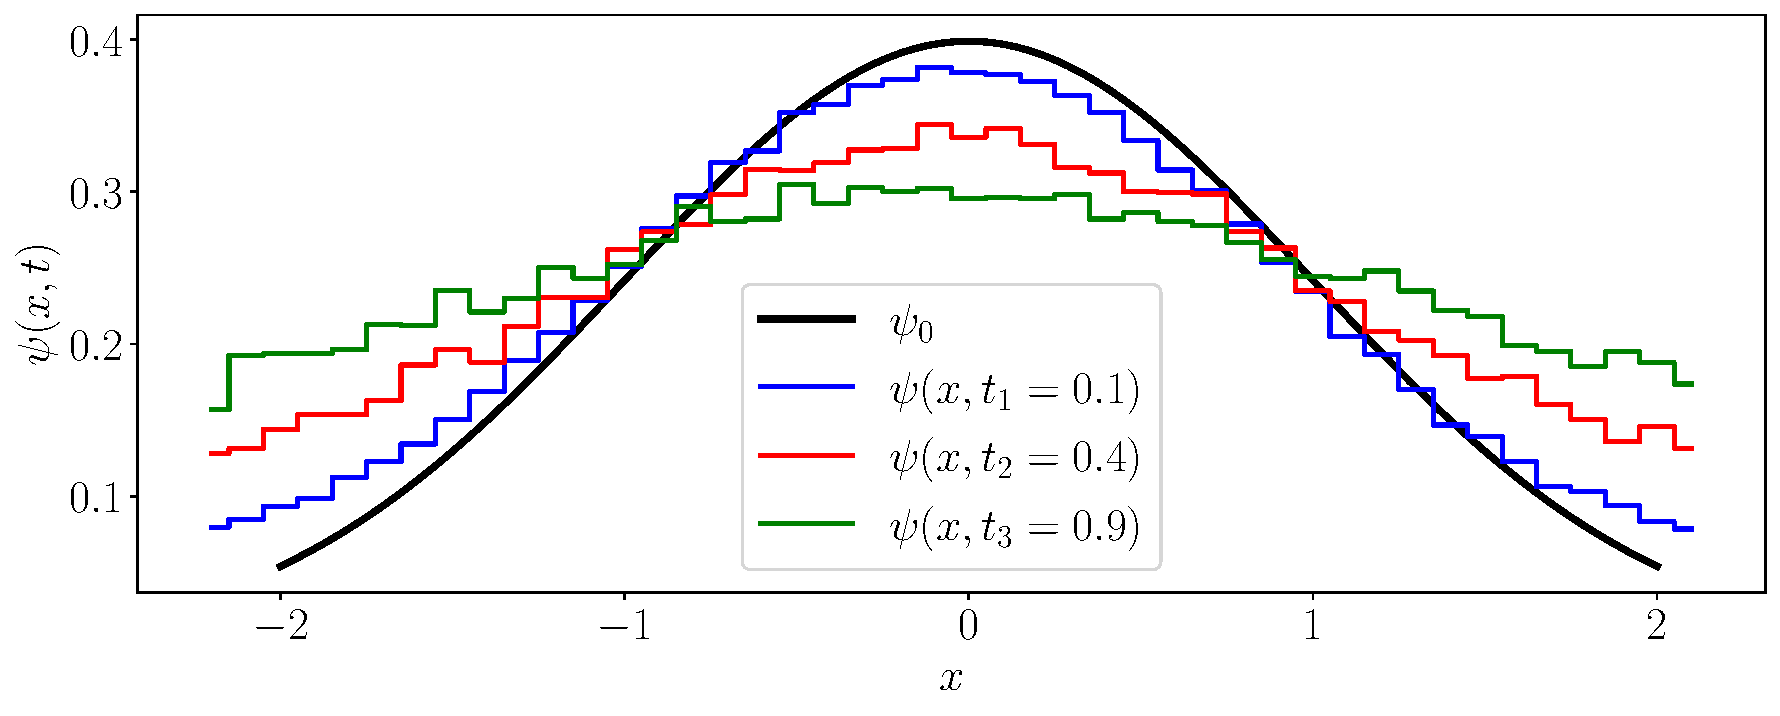
\includegraphics[width = \linewidth]{Chapter2/Figs/Raster/fkac_vs_fplanck_bottom.pdf}}
	
	\caption[Feynman-Kac for a 1D free particle]{\textbf{Feynman-Kac for a 1D free particle.} \textbf{top:} $N=400$ Brownian walks starting from different $x_0$, the color signifies initial position. In order to evaluate $\psi$ between $x-\frac{\delta x}{2}$ and $x+\frac{\delta x}{2}$ at some time $t$ we must first find Brownian paths that end there. \textbf{middle:} The paths that pass through at $x \in (1.5, 1.6)$ (blue) and through $x \in (-0.4,-0.3)$ (red) are colored, others are left in grey. \textbf{bottom:} Time evolution of the initial condition $\psi_{0} = \frac{1}{\sqrt{2 \pi}} e^{-\frac{1}{2} x^{2}}$, by estimating ${\mathbb{E}}\left[\psi\left(X_{0}, 0\right)\right]$ from the filtered paths at each timestep.}
	\label{fig:fk_1d_example}
\end{figure}
This simple case, does not involve the potential $V(x)$. The role of the potential in the Feynman-Kac formula is to weight the Brownian paths, in turn defining the Feynman-Kac \emph{path measure} $\mathbb{P}_{\mathrm{FK}}$. A path measure is simply a measure on the path space and the Feynman-Kac measure is related to the Brownian measure $\mathbb{P}_{0}$ by the \emph{Radon-Nykodym} derivative
\begin{equation}
	\frac{\mathrm{d} \mathbb{P}_{\mathrm{FK}}}{\mathrm{d} \mathbb{P}_{0}}=\mathcal{N} \exp \left(-\int V\left(X_{t}\right) d t\right),
\end{equation}
where $\mathcal{N}$ is a normalizing constant. Intuitively we can understand the measure as assigning more weight to Brownian paths that spend more time in the attractive region ($V(x) < 0$) than in repulsive regions ($V(x) > 0$), this is illustrated in Fig.~\ref{fig:fkac_measure_reweight}.
\begin{figure}[H]
	\centering
	\subfloat{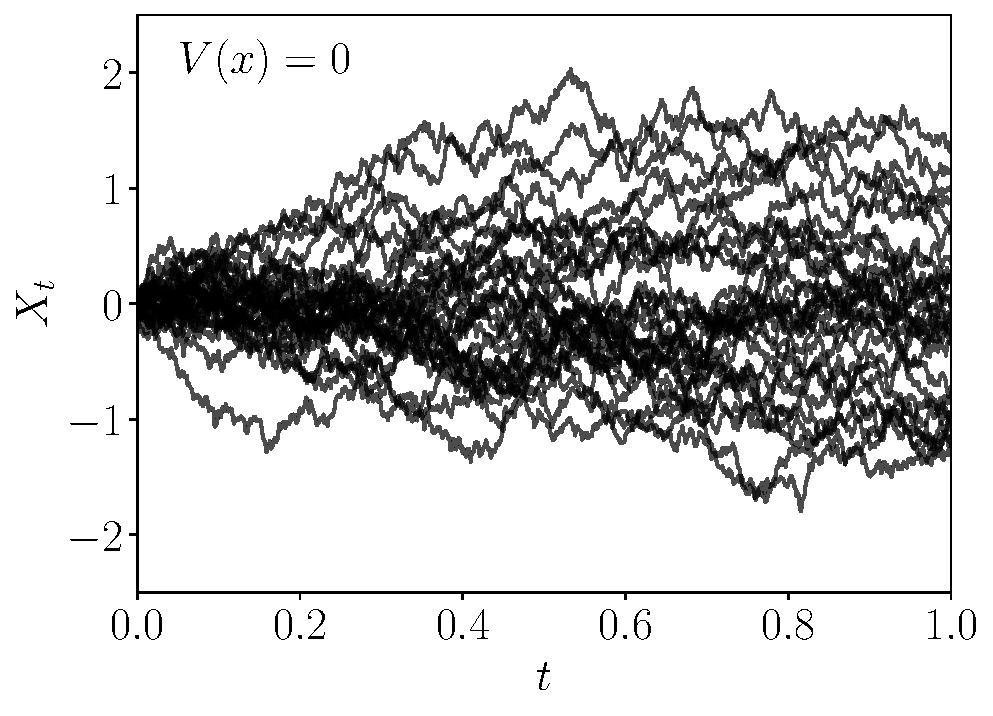
\includegraphics[width=0.5\linewidth]{Chapter2/Figs/Raster/reweight1.pdf}}
	\subfloat{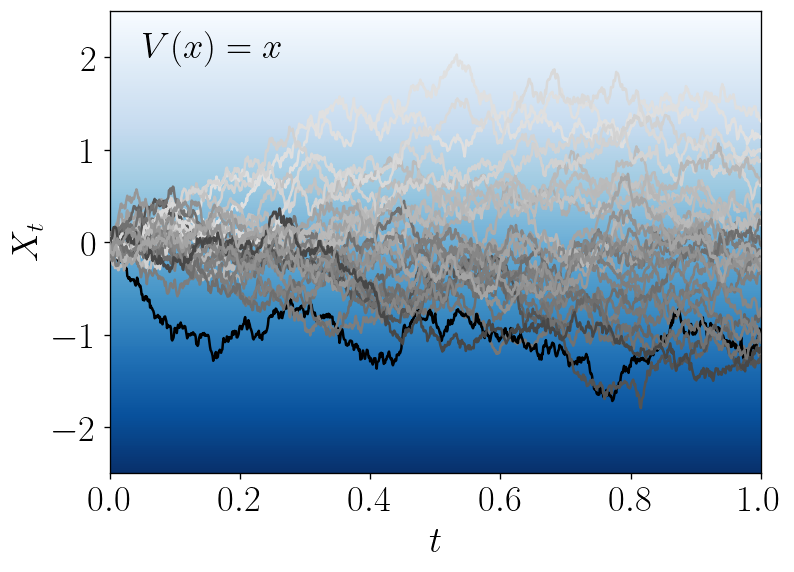
\includegraphics[width=0.5\linewidth]{Chapter2/Figs/Raster/reweight2.png}}
	\caption[Feynman-Kac measure in a linear potential]{\textbf{Feynman-Kac measure in a linear potential.} 
		\textbf{left:} $N=30$ Brownian paths. \textbf{right:} The paths colored by their likelihood under the Feynman-Kac measure with $V(x)=x$. }
	\label{fig:fkac_measure_reweight}
\end{figure}
Moreover, this new stochastic process is Markovian. This is crucial for our approach because of the connection with SDEs. In the continuous case we have discussed so far, the mapping between the Fokker-Planck equation and the Schr\" odinger equation is straightforward in terms of a similarity transform. Starting from the FP equation with drift $v(x)=-U^\prime(x)$ given as a gradient of some potential function $U(x)$ and its solution $\rho(t, x)$ 
\begin{equation}
	\frac{\partial \rho}{\partial t}=\mathcal{L}_{\mathrm{FP}} \rho=\frac{\partial}{\partial x}\left[\frac{\partial \rho}{\partial x}+U^{\prime}(x) \rho\right],
\end{equation}
we can define the function 
\begin{equation}
	\psi(x, t)=\frac{\rho(x, t)}{\sqrt{\rho_{0}(x)}},
\end{equation}
with $\rho_{0}$ being the stationary distribution of the FP equation
\begin{equation}
	\frac{\partial}{\partial x}\left[\frac{\partial \rho}{\partial x}+U^{\prime}(x) \rho\right] = 0 \quad \rightarrow \quad \rho_{0}(x) \propto \exp (-U(x)).
\end{equation}
Function $\psi(x, t)$ satisfies the imaginary time Schr\" odinger equation~\eqref{eq:imag_sch} with the Hamiltonian
\begin{equation}
	H=-\frac{\partial^{2}}{\partial x^{2}}-\frac{U^{\prime \prime}}{2}+\frac{U^{\prime 2}}{4}, 
\end{equation}
its ground state wavefunction is 
\begin{equation}
	\psi_{0}(x)=\sqrt{\rho_{0}(x)}.
\end{equation}
In other words, the quantum ground state probability distribution $|\psi_{0}|^2$ is the same as classical stationary distribution $\rho_{0}$ of the stochastic process $X_{t}$
\begin{equation}
	\mathrm{d} X_{t}=\mathrm{d} W_{t}+v\left(X_{t}\right) \mathrm{d} t,
\end{equation}
in the literature referred to as the \emph{Nelson's ground state process}~\cite{nelson1967dynamical, albeverio1977energy}. \hl{This connection serves as the backbone of our solution approach (revisit)}, as the ability to efficiently sample from the stochastic process is equivalent to sampling from the ground state of the quantum system. Even though the connection is simple, it comes with a caveat. Starting from the Schr\" odinger equation one needs to find the drift $v(x)$ and while the connection with the potential of the Hamiltonian is clear-cut in 1D, this is not the case in many-body systems, i.e. the \emph{inverse problem} of finding the stochastic process of a given Hamiltonian is difficult, and is one of the core problems approached in this thesis.

\newpage
\section{Stoquastic Hamiltonians and Lattice-model representations}
\label{subsec:fk-latt}
A similar connection between stochastic processes and the ground state exists in the discrete space, the difference being that instead of FP we have the Master equation


For a Markov process over discrete states, we can write the master equation as 
\begin{equation}
	\frac{\partial P_{j}}{\partial t}=\sum_{k \neq j}\left[\Gamma_{k \rightarrow j} P_{k}-\Gamma_{j \rightarrow k} P_{j}\right].
\end{equation}





\subsection{Single Particle on a Lattice}
\begin{equation}
	\partial_{t} \psi_{j}=\frac{1}{2}\left[\psi_{j+1}+\psi_{j-1}-2 \psi_{j}\right]+V_{j} \psi_{j}
\end{equation}

\begin{equation}
	\psi_{j}(t)=\underset{X \sim \mathrm{SRW} \text { with } X_{t}=j}{\mathbb{E}} \left[\exp \left(-\int_{0}^{t}  V\left(X_{\tau}, \tau\right) \mathrm{d} \tau \right) \psi_{X_{0}}(0)\right]
\end{equation}

\subsection{Transverse-field Ising model}

\subsection{Heisenberg model}
Heisenberg ferromagnet
\begin{equation}
	\hat H_{\mathrm{F}}=-\frac{1}{2} \sum_{j}\left[\hat{\sigma}_{j}^{x} \hat{\sigma}_{j+1}^{x}+\hat{\sigma}_{j}^{y} \hat{\sigma}_{j+1}^{y}+\hat{\sigma}_{j}^{z} \hat{\sigma}_{j+1}^{z}\right]
\end{equation}

The XY model.
\begin{equation}
	\begin{aligned} 
		\hat H_{X Y}=-\sum_{j}\left[\hat{\sigma}_{j}^{x} \hat{\sigma}_{j+1}^{x}+\hat{\sigma}_{j}^{y} \hat{\sigma}_{j+1}^{y}\right] &=H_{\mathrm{F}}+\frac{1}{2} \sum_{j} \hat{\sigma}_{j}^{z} \hat{\sigma}_{j+1}^{z} \\ 						&=-\mathcal{W}+\sum_{j}\left[n_{j}\left(1-n_{j+1}\right)+n_{j+1}\left(1-n_{j}\right)\right] 
	\end{aligned}
\end{equation}

\begin{equation}
	\psi_{s_{1: N}}(t)=\underset{\Sigma_{[0, t]} \sim \operatorname{SEP} \text{ with } \Sigma_{t}=s_{1: N}}{\mathbb{E}}
	\left[\exp \left(-\int_{0}^{t} d t^{\prime} \sum_{j}\left[n_{j}\left(1-n_{j+1}\right)+n_{j+1}\left(1-n_{j}\right)\right]\right) \psi_{\Sigma_{0}}(0)\right]
\end{equation}

\subsection{Bose-Hubbard model}


%********************************** % ??? Section  *************************************
\newpage
\section{Quantum Mechanics, Control and loss functions}

\subsection{Continuous space}

\subsection{Discrete space}

\begin{figure}
	\centering
	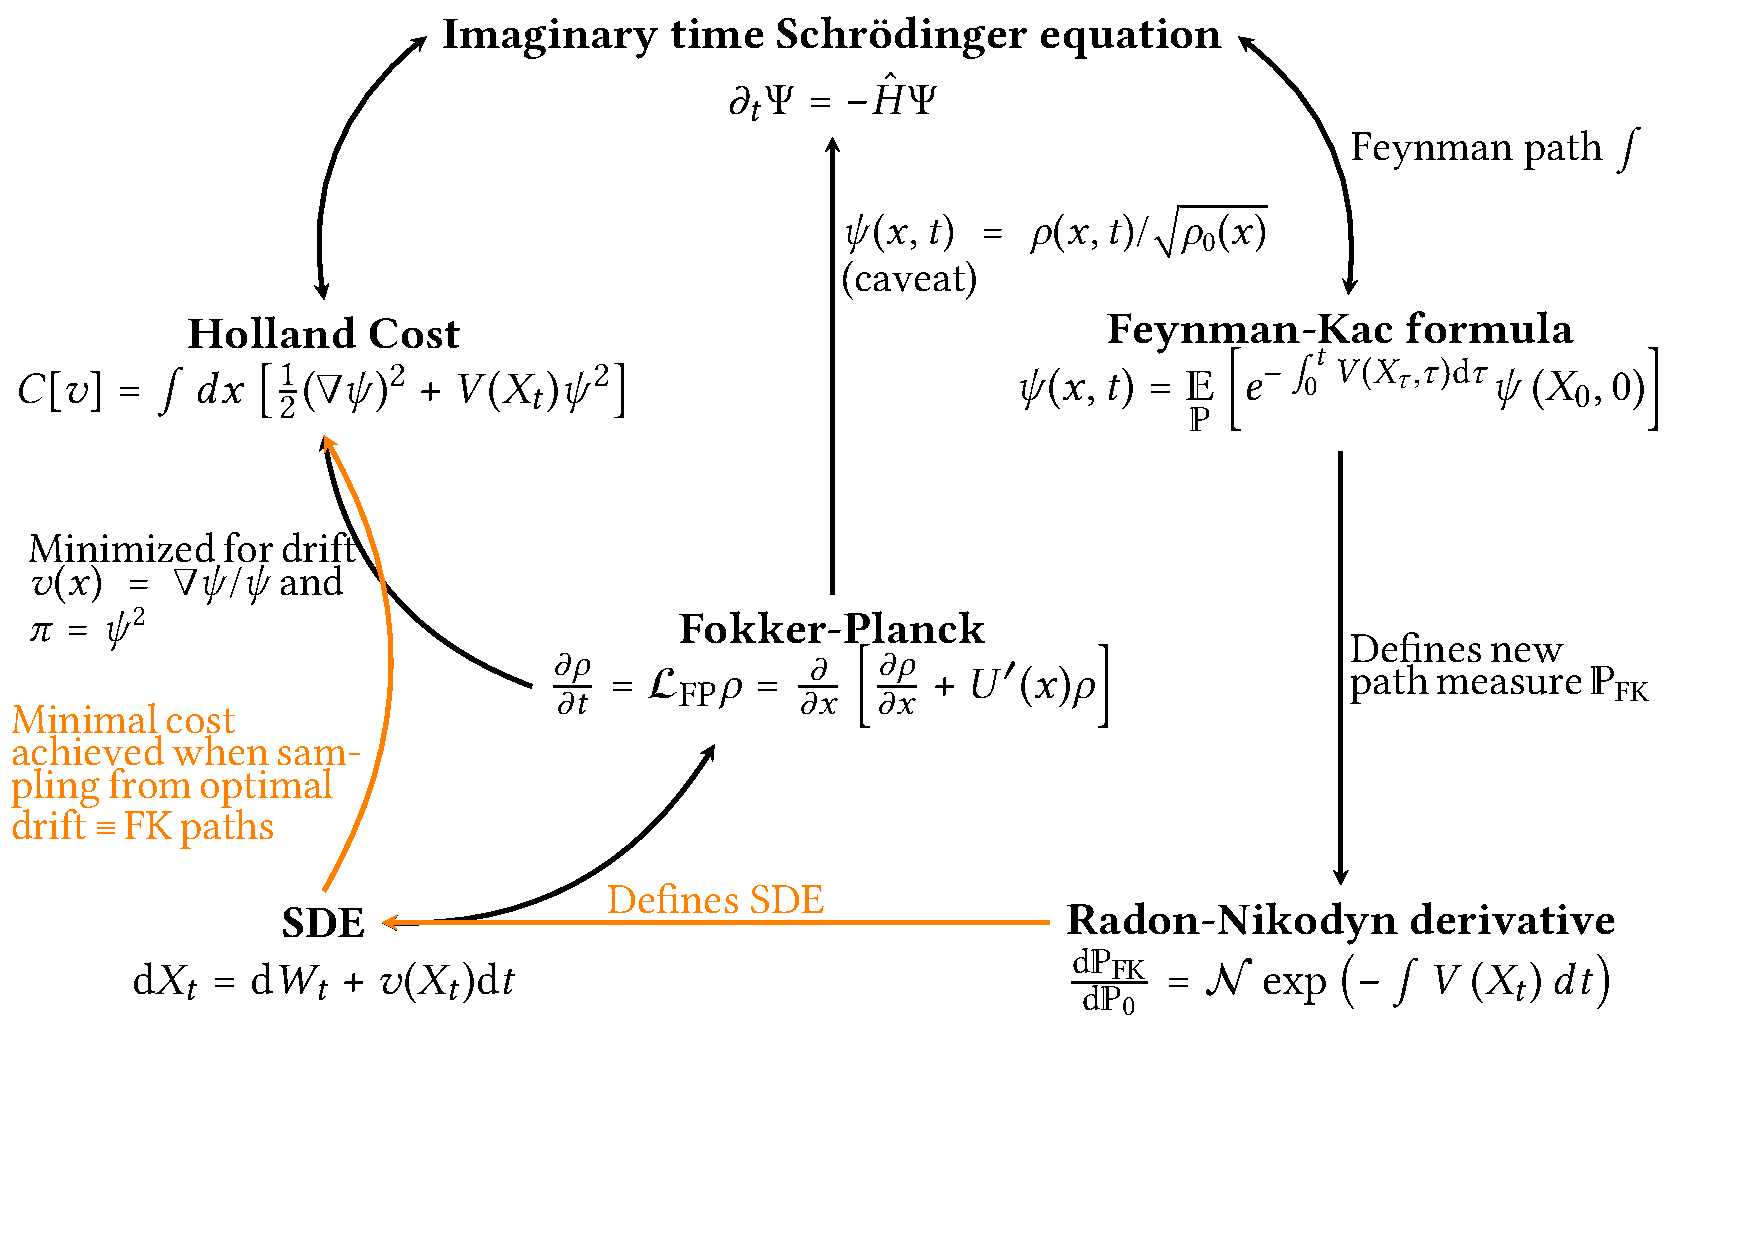
\includegraphics[angle=90, width=\linewidth]{Diagrams/bp/bp-c5}
	\caption[QM, stochastic processes and optimal control]{\textbf{QM, stochastic processes and optimal control}}
	\label{fig:bp-c5}
\end{figure}



%********************************** % Ch3 Nomenclature *************************************
\nomenclature[z-sde]{SDE}{Stochastic Differential Equations}
\nomenclature[z-fp]{FP}{Fokker-Planck}